\section{Experiments}
\label{sec: experiments}

\subsection{Evaluation Protocols}
\label{subsec: evaluation_protocols}
Allowing models to think freely can enhance performance but often results in lengthy responses. 
Current rule-based scorers are only effective with specific short formats, making it difficult to evaluate longer responses. Therefore, we need an \emph{answer extractor} (GPT4o) to convert detailed responses into concise ones. Following MATHVISTA~\cite{MATHVISTA} and MMLongBench-Doc~\cite{MMLongBench-Doc}, we implement a three-stage protocol: \emph{response generation}, \emph{answer extraction}, and \emph{score calculation}. In the \emph{score calculation} stage, we divide scores into five categories (\emph{Integer}, \emph{Float}, \emph{String}, \emph{List}, and \emph{None}). Different from MMLongBench-Doc, we adopt a softer and more reasonable scoring standard. See \Cref{xsec:experimental_details} for more details.

\subsection{Experimental Setup}
\label{subsec: experimental_setup}
\textbf{Models} We divide the experiments into two categories: \textbf{text-input} and \textbf{image-input}. For text-input configuration, document texts parsed by OCR engines are input into LLMs/LVLMs.
We conduct our experiments on both open-source and closed-source
models across 26 different configurations.

\noindent\textbf{Input Paradigm}
The documents in our \benchName~have a max of 150 pages, and most of models are unable to fully process the context to obtain the answer due to GPU memory or interface limitations. Therefore, similar to the \textbf{merge} method used in previous benchmarks~\cite{MMLongBench-Doc}, we design the \textbf{cut-off} paradigm for the evaluation of current models.

For LVLMs, we cut 30 continuous pages around the answer evidences from the original PDF-formatted document, and feed the converted images into the models. 
Details of selection rules are in \Cref{xsubsec:rules_of_images_selection}.
As for LLMs, we input the texts parsed by OCR engines, including PyMuPDF and Docmind.

\noindent\textbf{Other Configurations}
We assess the proprietary models using API resources, while the evaluation of the open-source models is conducted on H20 machines with 96G memory. To reduce variance, we set the temperature coefficient to 0.0 when generating free-form response and extracting short answer.

%\vfill
\begin{table*}[t]
    \centering
    \resizebox{\textwidth}{!}{
    \begin{tabular}{@{}l@{\hspace{1mm}}c|c@{\hspace{1mm}}c@{\hspace{1mm}}c@{\hspace{1mm}}c@{\hspace{1mm}}|c@{\hspace{1mm}}|c@{\hspace{1mm}}c@{\hspace{1mm}}c@{\hspace{1mm}}c@{\hspace{1mm}}|c@{\hspace{1mm}}|c@{\hspace{1mm}}c@{\hspace{1mm}}c@{\hspace{1mm}}c@{\hspace{1mm}}|c@{\hspace{1mm}}|c@{\hspace{1mm}}c@{\hspace{1mm}}c@{\hspace{1mm}}c@{\hspace{1mm}}|c@{\hspace{1mm}}|c@{\hspace{1mm}}c@{\hspace{1mm}}c@{\hspace{1mm}}c@{\hspace{1mm}}|c@{\hspace{1mm}}|c@{}}
    
        \toprule
        
        \multirow{4}{*}{\textbf{Model}} & \multirow{4}{*}{\textbf{Size}} & \multicolumn{10}{c|}{\textbf{Understanding}} & \multicolumn{10}{c|}{\textbf{Reasoning}} & \multicolumn{5}{c|}{\textbf{\Locating}} & \multirow{3}{*}{\textbf{Total}} \\
        
        & & \multicolumn{5}{c}{single-page} & \multicolumn{5}{c|}{multi-page} & \multicolumn{5}{c}{single-page} & \multicolumn{5}{c|}{multi-page} & \multicolumn{5}{c|}{cross-element} & \\
        
        & & TXT & LAY & FIG & TAB & \textcolor{blue}{all} & TXT & LAY & FIG & TAB & \textcolor{blue}{all} & TXT & LAY & FIG & TAB & \textcolor{blue}{all} & TXT & LAY & FIG & TAB & \textcolor{blue}{all} & CTi & CTa & PTi & FTa & \textcolor{blue}{all} & \\
        
        & & 259 & 91 & 94 & 263 & \textcolor{blue}{612} & 443 & 172 & 174 & 115 & \textcolor{blue}{631} & 40 & 12 & 28 & 98 & \textcolor{blue}{158} & 115 & 40 & 85 & 69 & \textcolor{blue}{229} & 201 & 126 & 137 & 231 & \textcolor{blue}{695} & 2325\\
        
        \midrule
        
        \multicolumn{28}{c}{\textit{OCR (PyMuPDF\footnotemark[4]) + Large Language Models (LLMs)} } \\
        
        \midrule
        
        {\textcolor{gray}{\textit{Open-source Models}}} \\
        
        LLaVA-Next-Interleave & 7B & 23.0 & 23.8 & 11.8 & 16.7 & \textcolor{blue}{19.5} & 36.2 & 32.3 & 25.0 & 29.2 & \textcolor{blue}{33.1} & 9.4 & 14.5 & 3.6 & 8.2 & \textcolor{blue}{8.7} & 27.3 & 15.0 & 20.8 & 23.3 & \textcolor{blue}{23.0} & 6.4 & 4.9 & 7.8 & 2.6 & \textcolor{blue}{5.8} & 18.7\\
        
        LLaVA-OneVision & 7B & 27.0 & 21.8 & 18.7 & 17.8 & \textcolor{blue}{22.7} & 43.1 & 37.6 & 33.6 & 33.4 & \textcolor{blue}{39.1} & 14.4 & 39.8 & 9.4 & 8.2 & \textcolor{blue}{10.4} & 31.9 & 25.0 & 29.0 & 20.5 & \textcolor{blue}{27.0} & 13.8 & 1.8 & 12.2 & 14.6 & \textcolor{blue}{11.2} & 23.3\\
        
        LLaVA-OneVision-Chat & 7B & 28.6 & 22.8 & 25.4 & 19.4 & \textcolor{blue}{24.6} & 43.0 & 36.3 & 35.4 & 31.0 & \textcolor{blue}{38.6} & 14.4 & 39.6 & 14.3 & 10.0 & \textcolor{blue}{12.4} & 31.2 & 20.0 & 28.0 & 22.4 & \textcolor{blue}{26.7} & 16.3 & 2.7 & 16.7 & 16.4 & \textcolor{blue}{14.0} & 24.6\\
        
        Qwen2-VL & 7B & 29.4 & 24.8 & 20.2 & 19.8 & \textcolor{blue}{24.5} & 42.3 & 36.6 & 33.6 & 33.3 & \textcolor{blue}{38.1} & 16.9 & 31.4 & 17.9 & 8.2 & \textcolor{blue}{12.5} & 32.0 & 22.5 & 33.8 & 23.7 & \textcolor{blue}{29.4} & 17.5 & 3.0 & 17.9 & 17.0 & \textcolor{blue}{14.9} & 25.0\\
        
        Qwen2.5-Instruct & 7B & 27.1 & 29.4 & 21.4 & 21.9 & \textcolor{blue}{24.7} & 36.5 & 32.9 & 33.8 & 28.0 & \textcolor{blue}{34.3} & 12.4 & 24.5 & 28.6 & 17.3 & \textcolor{blue}{18.3} & 32.0 & 32.5 & 29.2 & 24.2 & \textcolor{blue}{27.4} & 31.3 & 7.7 & 13.5 & 28.2 & \textcolor{blue}{20.5} & 25.9\\
        
        
        Qwen2.5-Instruct & 14B & 29.8 & 22.8 & 23.1 & 24.3 & \textcolor{blue}{26.4} & 38.4 & 34.6 & 37.4 & 33.5 & \textcolor{blue}{36.1} & 21.9 & 39.8 & 32.1 & 19.4 & \textcolor{blue}{21.4} & 29.3 & 35.0 & 22.1 & 22.7 & \textcolor{blue}{25.6} & 34.9 & 14.6 & 16.8 & 29.7 & \textcolor{blue}{24.2} & 27.9\\
        
        Qwen2.5-Instruct & 32B & 28.8 & 23.9 & 24.8 & 24.7 & \textcolor{blue}{26.6} & 34.9 & 32.6 & 31.3 & 36.0 & \textcolor{blue}{33.4} & 22.5 & 33.3 & 35.7 & 15.3 & \textcolor{blue}{20.3} & 31.1 & \colorbox{firstBest}{\textbf{40.0}} & 32.7 & 25.3 & \textcolor{blue}{29.4} & 33.5 & 23.1 & 28.5 & 31.2 & \textcolor{blue}{29.5} & 29.2\\
        
        Qwen2.5-Instruct & 72B & 31.9 & 30.3 & 23.3 & 25.3 & \textcolor{blue}{28.3} & 42.3 & 39.7 & 35.1 & 34.6 & \textcolor{blue}{39.4} & 22.5 & 25.0 & 35.7 & 15.3 & \textcolor{blue}{20.2} & \colorbox{firstBest}{\textbf{38.0}} & 39.9 & 32.6 & 26.7 & \textcolor{blue}{32.0} & 36.2 & 21.8 & 38.6 & 35.3 & \textcolor{blue}{34.2} & 32.9\\

        {\textcolor{gray}{\textit{Proprietary Models}}} \\
        
        Qwen-Max & - & 31.4 & 31.1 & 24.0 & 22.5 & \textcolor{blue}{27.1} & 40.0 & 35.3 & 33.5 & 34.8 & \textcolor{blue}{37.0} & 22.5 & 25.0 & 32.1 & 14.3 & \textcolor{blue}{19.0} & 31.9 & 37.5 & 31.5 & 22.9 & \textcolor{blue}{28.3} & 37.9 & 25.6 & 38.3 & 29.1 & \textcolor{blue}{34.0} & 31.4\\

        Gemini-1.5-Pro & - & 29.4 & 31.8 & 25.2 & 25.8 & \textcolor{blue}{27.8} & 41.3 & 40.3 & 35.5 & 32.0 & \textcolor{blue}{38.6} & 21.9 & 23.1 & 28.6 & 20.4 & \textcolor{blue}{21.4} & 31.9 & \colorbox{firstBest}{\textbf{40.0}} & \colorbox{firstBest}{\textbf{36.2}} & 24.3 & \textcolor{blue}{30.4} & 39.2 & 21.3 & 32.2 & 35.1 & \textcolor{blue}{32.8} & 32.0\\
        
        Qwen-VL-Max & - & \colorbox{firstBest}{\textbf{37.2}} & \colorbox{firstBest}{\textbf{37.0}} & 29.1 & 26.3 & \colorbox{firstBest}{\textcolor{blue}{\textbf{32.0}}} & \colorbox{firstBest}{\textbf{45.4}} & 44.1 & \colorbox{firstBest}{\textbf{39.9}} & \colorbox{firstBest}{\textbf{44.5}} & \colorbox{firstBest}{\textbf{\textcolor{blue}{43.3}}} & \colorbox{firstBest}{\textbf{28.7}} & \colorbox{firstBest}{\textbf{66.2}} & \colorbox{firstBest}{\textbf{45.8}} & 20.4 & \textcolor{blue}{26.8} & 37.1 & 37.5 & 33.8 & 27.1 & \textcolor{blue}{32.1} & 25.5 & 13.9 & 34.4 & 30.4 & \textcolor{blue}{27.3} & 33.3\\
        
        GPT-4o & - & 33.5 & 29.6 & 27.4 & 27.0 & \textcolor{blue}{30.4} & 42.6 & 42.7 & 38.0 & 33.5 & \textcolor{blue}{40.2} & 27.5 & 25.0 & 42.9 & 21.4 & \textcolor{blue}{25.9} & 33.7 & 37.5 & 31.5 & 25.6 & \textcolor{blue}{30.0} & \colorbox{firstBest}{\textbf{42.5}} & 24.1 & 40.8 & 35.6 & \textcolor{blue}{37.2} & 34.7\\
        
        O1-preview & - & 33.5 & 31.3 & \colorbox{firstBest}{\textbf{29.9}} & \colorbox{firstBest}{\textbf{29.6}} & \textcolor{blue}{31.1} & 41.7 & \colorbox{firstBest}{\textbf{45.0}} & 38.5 & 39.2 & \textcolor{blue}{40.1} & 22.5 & 33.3 & \colorbox{firstBest}{\textbf{45.8}} & \colorbox{firstBest}{\textbf{24.5}} & \colorbox{firstBest}{\textbf{\textcolor{blue}{27.1}}} & 34.9 & 37.5 & 29.2 & \colorbox{firstBest}{\textbf{38.6}} & \colorbox{firstBest}{\textbf{\textcolor{blue}{34.1}}} & 39.3 & \colorbox{firstBest}{\textbf{26.6}} & \colorbox{firstBest}{\textbf{44.9}} & \colorbox{firstBest}{\textbf{37.8}} & \colorbox{firstBest}{\textbf{\textcolor{blue}{38.6}}} & \colorbox{firstBest}{\textbf{35.8}}\\

        \midrule
        
        \multicolumn{28}{c}{\textit{Large Vision Language Models (LVLMs)} } \\
        
        \midrule
        
        {\textcolor{gray}{\textit{Open-source Models}}} \\
        
        InternLM-XC2.5 & 7B & 2.9 & 3.0 & 2.7 & 2.1 & \textcolor{blue}{2.7} & 5.5 & 5.3 & 3.2 & 2.7 & \textcolor{blue}{4.5} & 2.5 & 8.3 & 0.0 & 0.0 & \textcolor{blue}{0.6} & 3.5 & 2.5 & 1.2 & 1.3 & \textcolor{blue}{2.6} & 0.6 & 0.4 & 0.5 & 1.3 & \textcolor{blue}{0.7} & 2.4\\

        mPLUG-DocOwl2 & 7B & 6.2 & 6.9 & 4.6 & 3.5 & \textcolor{blue}{5.4} & 11.6 & 10.7 & 10.6 & 8.8 & \textcolor{blue}{9.9} & 2.5 & 8.3 & 0.0 & 1.0 & \textcolor{blue}{1.3} & 7.4 & 7.5 & 4.7 & 4.2 & \textcolor{blue}{5.5} & 2.4 & 0.0 & 1.8 & 2.4 & \textcolor{blue}{1.8} & 5.3 \\
        
        Pixtral & 12B & 10.1 & 8.2 & 6.7 & 4.6 & \textcolor{blue}{7.5} & 10.2 & 8.6 & 5.5 & 7.2 & \textcolor{blue}{8.4} & 2.7 & 8.9 & 0.0 & 0.0 & \textcolor{blue}{0.7} & 10.0 & 5.0 & 4.6 & 2.5 & \textcolor{blue}{5.8} & 3.7 & 1.3 & 1.9 & 2.2 & \textcolor{blue}{2.4} & 5.6\\
        
        Llama-3.2 & 11B & 11.9 & 9.9 & 13.1 & 8.1 & \textcolor{blue}{10.3} & 15.5 & 16.0 & 12.4 & 13.0 & \textcolor{blue}{15.3} & 2.5 & 8.3 & 10.7 & 6.1 & \textcolor{blue}{7.0} & 13.0 & 15.0 & 9.3 & 6.4 & \textcolor{blue}{11.0} & 3.0 & 1.4 & 3.8 & 1.6 & \textcolor{blue}{2.7} & 9.2\\

        LLaVA-Next-Interleave & 7B & 19.7 & 17.1 & 8.6 & 8.1 & \textcolor{blue}{14.0} & 30.3 & 25.4 & 19.7 & 16.6 & \textcolor{blue}{26.3} & 7.5 & 16.7 & 10.1 & 5.1 & \textcolor{blue}{6.9} & 21.4 & 12.5 & 19.9 & 8.5 & \textcolor{blue}{17.2} & 6.6 & 1.1 & 3.7 & 2.4 & \textcolor{blue}{3.8} & 14.1\\
        
        LLaVA-OneVision & 7B & 28.6 & 32.4 & 19.2 & 14.6 & \textcolor{blue}{22.3} & 36.7 & 37.1 & 28.1 & 23.5 & \textcolor{blue}{33.7} & 10.7 & 22.9 & 6.5 & 6.0 & \textcolor{blue}{7.6} & 26.4 & 20.0 & 24.0 & 12.2 & \textcolor{blue}{22.6} & 17.7 & 9.2 & 6.8 & 25.5 & \textcolor{blue}{14.1} & 22.0\\
        
        LLaVA-OneVision-Chat & 7B & 29.5 & 34.1 & 26.0 & 17.9 & \textcolor{blue}{24.8} & 36.9 & 38.4 & 34.5 & 26.9 & \textcolor{blue}{36.0} & 6.9 & 14.5 & 6.5 & 8.2 & \textcolor{blue}{8.0} & 31.8 & 22.5 & 29.3 & 16.5 & \textcolor{blue}{26.6} & 22.5 & 9.9 & 13.6 & 29.7 & \textcolor{blue}{18.7} & 25.0\\
        
        Qwen2-VL & 7B & 37.9 & 37.2 & 30.0 & 29.8 & \textcolor{blue}{33.4} & 43.8 & 38.0 & 37.8 & 33.5 & \textcolor{blue}{40.2} & 19.0 & 54.9 & 21.4 & 17.2 & \textcolor{blue}{19.3} & 33.2 & 22.5 & 34.5 & 16.5 & \textcolor{blue}{28.6} & 25.7 & 22.1 & 17.6 & 27.0 & \textcolor{blue}{22.6} & 30.6\\
        
        {\textcolor{gray}{\textit{Proprietary Models}}} \\

        Qwen-VL-Max & - & 61.1 & 54.5 & 58.2 & 53.7 & \textcolor{blue}{57.7} & 63.0 & 57.2 & 56.1 & 53.3 & \textcolor{blue}{60.0} & 44.1 & \colorbox{firstBest}{\textbf{66.6}} & 57.1 & 38.6 & \textcolor{blue}{44.0} & 45.8 & 42.5 & 38.5 & 41.0 & \textcolor{blue}{43.8} & 25.4 & 16.7 & 47.5 & 49.8 & \textcolor{blue}{36.0} & 49.5\\
        
        Gemini-1.5-Pro & - & 54.8 & 57.2 & 60.1 & 48.8 & \textcolor{blue}{52.8} & 61.4 & 56.9 & 54.2 & 51.8 & \textcolor{blue}{58.4} & 37.7 & 57.9 & 46.4 & 31.3 & \textcolor{blue}{35.9} & 53.4 & 52.5 & 47.8 & 40.4 & \textcolor{blue}{48.6} & 48.4 & 18.9 & 46.7 & 68.1 & \textcolor{blue}{46.4} & 50.9\\
        
        GPT-4o & - & \colorbox{firstBest}{\textbf{71.1}} & \colorbox{firstBest}{\textbf{67.5}} & \colorbox{firstBest}{\textbf{68.5}} & \colorbox{firstBest}{\textbf{66.4}} & \colorbox{firstBest}{\textbf{\textcolor{blue}{68.6}}} & \colorbox{firstBest}{\textbf{70.1}} & \colorbox{firstBest}{\textbf{67.4}} & \colorbox{firstBest}{\textbf{69.1}} & \colorbox{firstBest}{\textbf{63.8}} & \colorbox{firstBest}{\textbf{\textcolor{blue}{68.6}}} & \colorbox{firstBest}{\textbf{56.7}} & \colorbox{firstBest}{\textbf{66.6}} & \colorbox{firstBest}{\textbf{70.8}} & \colorbox{firstBest}{\textbf{49.5}} & \colorbox{firstBest}{\textbf{\textcolor{blue}{55.7}}} & \colorbox{firstBest}{\textbf{67.3}} & \colorbox{firstBest}{\textbf{55.0}} & \colorbox{firstBest}{\textbf{61.7}} & \colorbox{firstBest}{\textbf{61.1}} & \colorbox{firstBest}{\textbf{\textcolor{blue}{62.8}}} & 50.7 & \colorbox{firstBest}{\textbf{40.1}} & \colorbox{firstBest}{\textbf{66.8}} & \colorbox{firstBest}{\textbf{78.5}} & \colorbox{firstBest}{\textbf{\textcolor{blue}{59.6}}} & \colorbox{firstBest}{\textbf{64.5}}\\

        \midrule
        \multicolumn{28}{c}{\textit{Human Baseline} } \\
        \midrule
        Human Experts & - & - & - & - & - & \textcolor{blue}{-} & - & - & - & - & \textcolor{blue}{87.2} & - & - & - & - & \textcolor{blue}{-} & - & - & - & - & \textcolor{blue}{81.3} & - & - & - & - & \textcolor{blue}{81.6} & 84.8 \\
        
        \bottomrule
    \end{tabular}}
    \caption{Generalized accuracy scores(0\textasciitilde1) on \benchName. There are 3 types of tasks: (U)nderstanding, (R)easoning, and (L)ocating. There are 4 types of evidence elements: pure text(TXT), layout(LAY), chart \& image(FIG), and table(TAB). There are 3 types of evidence pages/elements: single-page(SP), multi-page(MP), and cross-element(CE). Cross-element means at least two element types in the evidence(\eg, chart and table). CTi: Cross-Title, CTa: Cross-Table, PTi: Para-Title, FTa: Figure-Table. The highest scores among models in each section are highlighted in \colorbox{firstBest}{\textbf{green}}. \textit{Human baselines} are obtained from 102 uniformly distributed samples.}
    \label{tab:main_results_1}
    \vspace{-5mm}
\end{table*}

\subsection{Main Results}
\label{subsec: main_results}
As shown in \Cref{tab:main_results_1} and \Cref{tab:main_results_2}, we calculate generalized accuracy scores to assess model capabilities. Regarding LVLMs, we draw the following conclusions: (1) \textbf{Highest Scoring Model}: Only GPT-4o meets the passing standard and scores highest at 64.5, indicating that our \benchName~presents significant challenges for current models. (2) \textbf{Comparison of Open-source and Closed-source models}: Proprietary models demonstrate better overall performance compared to open-source models. Among open-source models, only Qwen2-VL (score 30.6) and LLaVA-OneVision (scores 22.0 and 25.0) exceed a score of 20, while other models with fewer than 13B parameters fall below this threshold.


To compare the performance of models using text input versus image input, we included the O1-preview and Qwen2.5 series. The experimental results show that the overall scores of LLMs significantly lower than LVLMs, with the top LLM score trailing the top LVLM score by about 30 points. This gap is mainly because important document information is lost when parsed into plain text using PyMuPDF. Our dataset features numerous table-related and chart-related Q\&A pairs, and the loss of structural information hinders LLMs’ ability to extract critical evidence. These results highlights our \benchName~ as a benchmark for assessing the document structure parsing capability of LVLMs.



\subsubsection{Fine-Grained Analysis}
\label{subsubsec:multi-dimensional_analysis}

% 
\begin{figure*}[htbp]
    \centering
    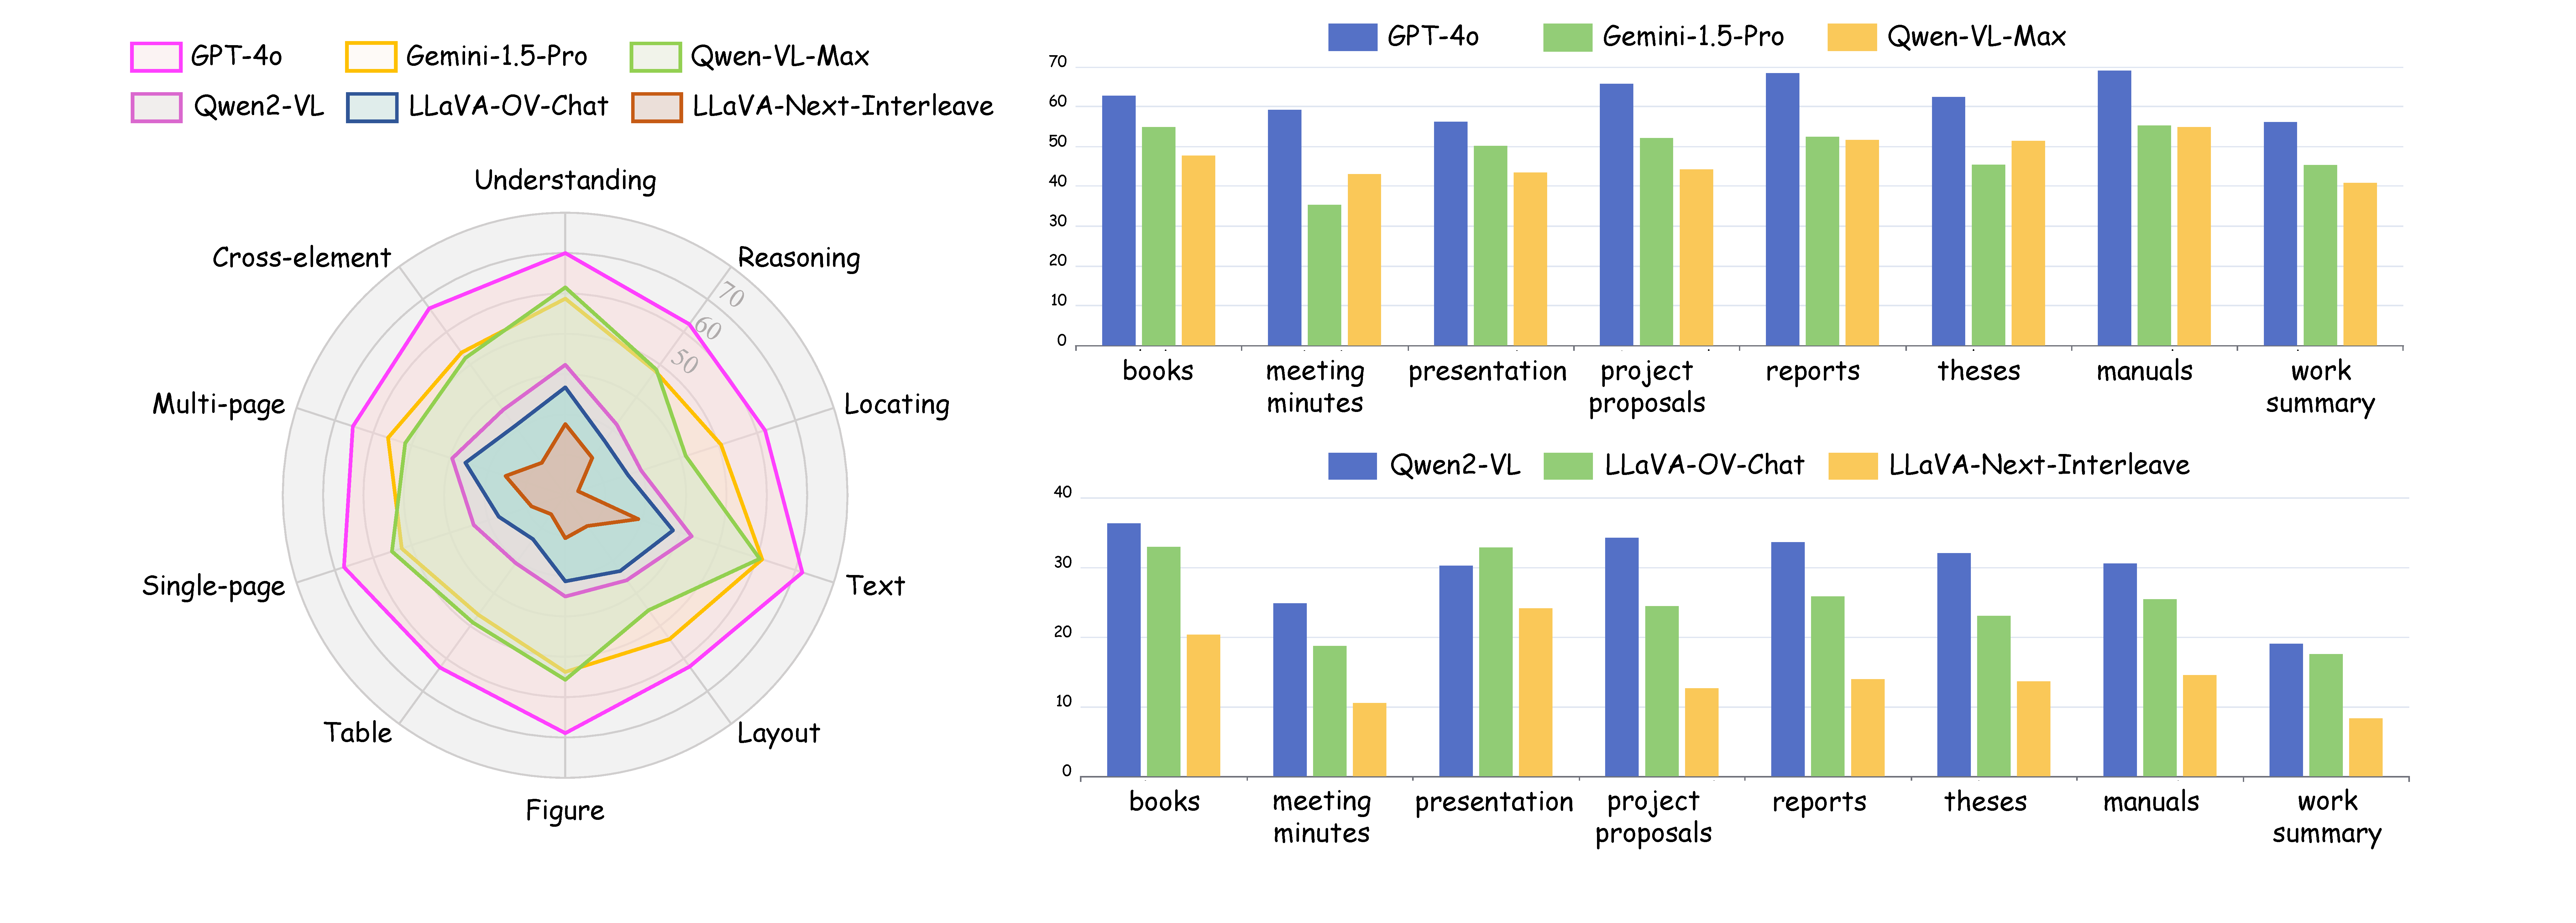
\includegraphics[width=\textwidth]{img/scores_6models.pdf} % 调整宽度
    \vspace{-0.5cm}
    \caption{Fine-grained Results. We choose 3 proprietary and 3 open-source models to conduct further analysis based on (left) \textbf{task types}, \textbf{document elements}, \textbf{evidence pages}, and (right) \textbf{document sources}.}
    \vspace{-0.2cm}
    \label{fig:fine_grained_results}
\end{figure*}

We include more fine-grained results in \Cref{tab:main_results_2} and \Cref{fig:fine_grained_results}, based on document sources, task categories, document elements, and evidence pages.

\noindent\textbf{Document Sources} 
As shown in \Cref{fig:fine_grained_results}, the models perform better on \emph{books}, \emph{reports}, \emph{manuals}, and \emph{project proposals}, likely due to their simpler layout, which facilitates key information extraction. Conversely, the models struggle with less common documents like \emph{meeting minutes} and \emph{work summary}, which have limited data.

\noindent\textbf{Task Type} 
Observations reveal: (1) Proprietary LVLMs perform comparably on reasoning and \locating~tasks, but image-to-text conversion impacts reasoning capabilities more severely. For instance, switching to text input, GPT-4o's reasoning scores drop by 31.6 points versus 22.4 points for \locating. (2) Strong models are balanced in reasoning and \locating, whereas weaker models perform poorly on \locating, suggesting a training focus on capabilities of understanding and reasoning over spatial and logical relationships in \locating~tasks.

\noindent\textbf{Document Elements} 
Models score highest on \emph{Text} questions and lowest on \emph{Table} ones, highlighting deficiencies in document structure parsing. \emph{Figure} and \emph{Layout} question types yield similar scores. Scores for cross-element tasks fall between single-page and multi-page QA, closely aligning with the overall assessment.


\noindent\textbf{Single-page vs Multi-page} 
Single-page QA accuracy is lower than multi-page QA. This reveals that answers for some questions can be gathered from multiple pages, thereby reducing the difficulty. However, models like GPT-4o and Qwen-VL-Max show lower accuracy on multi-page QA, revealing a contradiction where their scores on \locating~tasks in multi-page QA are lower, thus skewing overall performance.


\begin{table}[htbp]
    \centering
    \resizebox{0.5\textwidth}{!}{
    \begin{tabular}{@{}lc|cc|ccc@{}}
        \toprule
        \multirow{2}{*}{\textbf{Model}} & \multirow{2}{*}{\textbf{Size}} & \multicolumn{2}{c|}{\textbf{Image-input}} & \multicolumn{2}{c}{\textbf{Text-input}} \\
        & & cut-off & merge & pymupdf & docmind \\
        % & & 30 & All & 30 & 30 \\
        \midrule
        \textcolor{gray}{\textit{Open-source Models}} \\
        Qwen2-VL & 7B & 30.7 & 7.6\footnotemark[4] & 24.4 & 45.3 \\
        LLaVA-Next-Interleave & 7B & 12.6 & 10.9 & 16.9 & 29.7 \\
        LLaVA-OneVision-Chat & 7B & 24.1 & 14.0 & 23.0 & 39.1 \\
        
        \textcolor{gray}{\textit{Proprietary Models}} \\
        Gemini-1.5-Pro & - & 48.1 & -\footnotemark[5] & 34.0 & 64.8 \\
        GPT-4o & - & 64.4 & 44.9 & 36.5 & 66.2 \\
        O1-preview & - & - & - & 38.0 & 63.4 \\
        
        \bottomrule
    \end{tabular}
    }
    \caption{Comparison among different input paradigms on a subset of 20\% data.}
    \label{tab:results_in_different_input_formats}
    \vspace{-6mm}
\end{table}

\footnotetext[4]{363 out of 465 Q\&A pairs meet OOM problems with Qwen2-VL. We calculate normalized score on the size of 465.}
\footnotetext[5]{Not completed due to resource limitations.}



\subsection{Ablation of Input Paradigms}
\label{subsec: ablation_of_input_paradigms}

To explore the optimal input format in long document question-answering, we conduct ablation experiments across two image-input and two text-input paradigms. The image-input paradigms include: (1) \textbf{cut-off}, following the configuration detailed in \Cref{subsec: experimental_setup}, and (2) \textbf{merge}, where document images are combined from raw document lengths (50\textasciitilde150) into 20\textasciitilde30 new images. Further details can be found in \Cref{xsubsec:rules_of_images_merging}. 

We note that the table structure information significantly degrades when parsed by PyMuPDF, while the markdown-format table texts parsed by Docmind retain greater structural integrity. To assess the impact of structural information loss on model performance, we conducted experiments with two input types: (1) \textbf{text-input-docmind}, utilizing texts parsed by Docmind, and (2) \textbf{text-input-pymupdf}, utilizing texts parsed by PyMuPDF. The analysis of the results presented in \Cref{tab:results_in_different_input_formats} led us to the following conclusions:

\noindent\textbf{Text-input vs. Image-input:} 
The scores in the \emph{cut-off} paradigm are higher than that in the \emph{text-input-pymupdf} paradigm, but lower than that in the \emph{text-input-docmind} paradigm, indicating that this method can effectively extract table structure information, but it can be improved further. 

\noindent\textbf{Cut-off vs. Merge:}
The \emph{merge} method preserves a greater number of context tokens by concatenating multiple images, while the \emph{cut-off} method succeeds in acquiring prior information by shortening the context window. Experimental results suggest that the cut-off may yield better problem-solving capabilities than merging, providing insights for the future construction of multimodal Retrieval-Augmented Generation (RAG) systems.

\noindent\textbf{Impact of Structural Information:}
For proprietary models, performance utilizing Docmind is at least 25 points higher than that with PyMuPDF, while the disparity is 15 points for open-source models. The absence of table structure information significantly hampers the performance of both open-source and proprietary models.

